% !TeX spellcheck = en_US
\chapter{Evaluation}%
\label{sec:evaluation}

The overall goal of this project is to obtain a control law via reverse engineering the model dynamics to answers the following question: How must the~\glsxtrshort{aea} be set in relation to$~\gls{rho}$ to get a touchdown with the current state$~\begin{bmatrix} \gls{q} & \dot{\gls{q}} \end{bmatrix}^\textrm{T}$ so that the periodicity of the gait is preserved in the subsequent step? By simulating and analyzing the dynamics of the entire system, an attempt is made to deduce a control law. The ideal case would be to find a constant offset which, independent of the magnitude of the velocity vector$~\gls{v}_{CH}$, always leads to a periodic solution. \\

To find an answer to this question, the optimizer was left to find a solution as periodic as possible via the cost function from equation~\ref{eq:objective-function}. A preliminary sweep in a feasible range was performed considering$~\gls{GM}_h$ and$~\gls{theta-es}_{,~k}$ separately, in order to observe a tendency of their influence in the behavior of the system. Note that varying$~\gls{theta-es}_{,~k}$ does not increase the velocity significantly, however, increasing the gain of the hip motor$~\gls{GM}_h$ does, since this straightly affects the output voltage of the motors, but the system also becomes increasingly unstable, to the point where it is not able to walk anymore.$~\gls{theta-fs}_{,~k}$ was excluded from the sweep as it seems to have a much more erratic behavior. Additionally, since any deviation from$~\gls{theta-es}_{,~h}$ seemed to negatively affect the robustness of the system, this parameter was left at the default value of 5. \\

Finding appropriate initial parameters for a stable gait is one of the biggest challenges in modelling a spring-mass biped, which often turns out to be time-consuming and tedious. As it is not possible to analytically deduce the dependence of the stability of the system on the initial parameters, most of them have to be found through experiments. In addition, even small disturbances of the permissible parameters can quickly lead to instability of the entire system. In this project, most of the parameters were chosen according to appropriate experimental data from~\citeauthor*{Geng2006}~\cite{Geng2006} and the remaining ones were determined by sweeping within a reasonable range. The parameters obtained from the sweep consist of

\begin{align}
    \begin{cases}
        \gls{theta-es}_{,~k} = -4.25  \\
        \gls{theta-fs}_{,~h} =~\text{\glsxtrshort{aea}} = \frac{15}{1 + e^{0.2 \cdot \gls{rho} + 4}} - 25  \\
        \gls{GM}_h = 1.6
    \end{cases}      
    \label{eq:results}%
\end{align}
% \noindent

The resulting walking gait using the parameters from equation~\ref{eq:results} is summarized in table~\ref{tab:results}. The results of the performed~\glsxtrshort{mca} are summarized in table~\ref{tab:mca}.

\begin{table}[H]
    \caption{The results of the walking gait.} \label{tab:results}
    \begin{center}
        \begin{tabular}{ l|l|l|l }
            \textbf{Symbol}                             & \textbf{Description}              & \textbf{Value}    & \textbf{Unit}                         \\ [0.5ex]
            \hline \hline
            $\gls{x}_{\glsxtrshort{com},~end}$                & Distance covered                  & 15                &$~\left[\si{\metre}\right]$            \\
            $\gls{t}_{end}$                             & Time required                     & 18.8502           &$~\left[\si{\second}\right]$           \\
            $\overline{\gls{v}_{\glsxtrshort{com}_x}}$ & Average forward velocity          & 0.8379            &$~\left[\si{\metre\per\second}\right]$ \\
            $\gls{v}_{\glsxtrshort{com}_x,~max}$       & Maximum instantaneous velocity    & 1.7803            &$~\left[\si{\metre\per\second}\right]$ \\
            $\gls{v}_{\glsxtrshort{com}_x,~min}$       & Minimum instantaneous velocity    & -0.7106           &$~\left[\si{\metre\per\second}\right]$ \\
            $\gls{y}_{\glsxtrshort{com},~max}$                & Highest vertical displacement     & 0.2907            &$~\left[\si{\metre}\right]$            \\
            $\gls{y}_{\glsxtrshort{com},~min}$                & Lowest vertical displacement      & 0.2031            &$~\left[\si{\metre}\right]$  
        \end{tabular}
    \end{center}
\end{table}

\begin{table}[H]
    \caption{The results of the~\glsxtrlong{mca}.} \label{tab:mca}
    \begin{center}
        \begin{tabular}{ l|l|l|l }
            \textbf{Symbol}         & \textbf{Description}      & \textbf{Value}    & \textbf{Unit}                                     \\ [0.5ex]
            \hline \hline
            $\gls{Fr}$              & Froude number             & 0.2468            & -                                                 \\
            $\sqrt{\gls{Fr}}$       & Dimensionless velocity    & 0.4986            & -                                                 \\
            $\gls{Theta}$           & Average force angle       & 0.7285            & $\left[\si{\radian}\right]$                       \\
            $\gls{Lambda}$          & Average velocity angle    & 0.3704            & $\left[\si{\radian}\right]$                       \\
            $\gls{Phi}$             & Average collision angle   & 0.9855            & $\left[\si{\radian}\right]$                       \\
            \glsxtrshort{mcot}      & \glsdesc{mcot}            & 0.5226             & $\left[\si{\joule\per\metre\per\newton}\right]$   \\
            $\gls{kappa}$           & Collision fraction        & 0.8968            & -  
        \end{tabular}
    \end{center}
\end{table}

Compared to mammals from the literature, the~\glsxtrshort{mcot} of the robot is relatively high. Humans, for example, walk with~\glsxtrshort{mcot} $\approx 0.08$ and run with~\glsxtrshort{mcot} $\approx 0.28$~\cite{Lee2013}. Figure~\ref{fig:collision-based-analysis} shows~\gls{Theta},~\gls{Lambda} and~\gls{Phi} as a fraction of their sum in a ternary diagram. The filled circles indicate bipedal gaits and the filled squares indicate quadrupedal gaits. The color of the symbols indicate the collision fraction~\gls{kappa} with red indicating$~\kappa = 1$ and purple$~\kappa = 0$ (for spectrum of intermediate colors, see color scale at right).~\cite{Lee2013}

\begin{figure}[H]%
    \centering%
    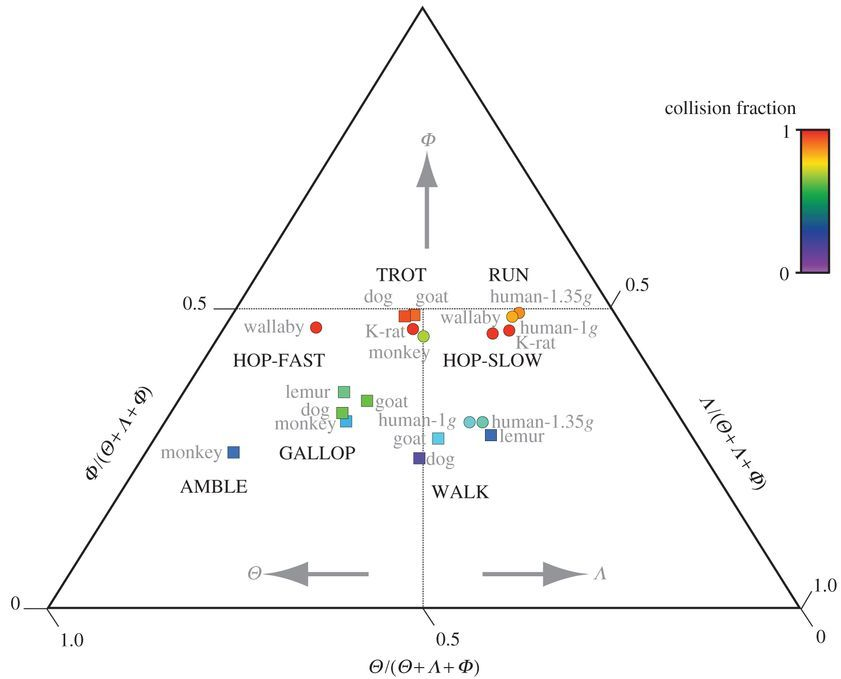
\includegraphics[width=\linewidth]{collision-based-analysis/ternary-diagram.png}
    \caption{The collision-based analysis of selected mammals from the literature.~\gls{Theta},~\gls{Lambda} and~\gls{Phi} are shown as a fraction of their sum in a ternary diagram. The filled circles indicate bipedal gaits and the filled squares indicate quadrupedal gaits. The color of the symbols indicate the collision fraction~\gls{kappa} with red indicating$~\kappa = 1$ and purple$~\kappa = 0$ (for spectrum of intermediate colors, see color scale at right). (Adapted from~\cite{Lee2013}, p. 6)}%
    \label{fig:collision-based-analysis}%
\end{figure}%
% \noindent

Figure~\ref{fig:velocity-vectors} shows the velocity vectors$~\gls{v}_{\glsxtrshort{com}}$ at touchdown (\subref{fig:velocity-vectors-touchdown}) and at~\glsxtrshort{vlo}$_{1}$ (\subref{fig:velocity-vectors-vlo}). At the beginning of the velocity vectors the leg position is shown schematically, where the hip, knee and ankle joints are drawn as circles. Accordingly, it can be seen that the robot performs the touchdown with a fully extended knee if$~\gls{GM}_h \geq 1.6$. With a$~\gls{GM}_h$ of 1.4, the swing leg of the robot is not fast enough to reach an extended knee at touchdown. The velocity vectors at touchdown are always in the fourth quadrant, which means that the robot has a positive horizontal forward velocity ($\gls{v}_{\glsxtrshort{com}_x} > 0\,\textrm{\si{\metre\per\second}}$) and a negative vertical velocity ($\gls{v}_{\glsxtrshort{com}_y} < 0\,\textrm{\si{\metre\per\second}}$), in other words, the torso falls forward and is caught by the swing leg at touchdown. The velocity vectors at~\glsxtrshort{vlo}$_{1}$ are always in the first quadrant, which means that the robot has a positive horizontal as well as vertical velocity ($\gls{v}_{\glsxtrshort{com}_x}~\land~\gls{v}_{\glsxtrshort{com}_y} > 0\,\textrm{\si{\metre\per\second}}$). A single step is completed when the swing leg attains ground contact and the~\glsxtrshort{com} is orthogonally above the second foot point ($\gls{x}_{\glsxtrshort{com}} = \gls{x}_{FP_2}$). The colors refer to the different motor gains, with red representing the lowest with$~\gls{GM}_h = 1.4$, and blue the highest with$~\gls{GM}_h = 1.8$. The angle of the velocity vector tends to get steeper the larger the motor gain$~\gls{GM}_h$,~\ie the faster the robot runs. A steeper velocity vector has more vertical than horizontal velocity and thus leads to a steeper angle of attack~\gls{alpha}.

\begin{figure}[H]%
    \centering%
    \begin{subfigure}[t]{0.8\linewidth}%
        \centering%
        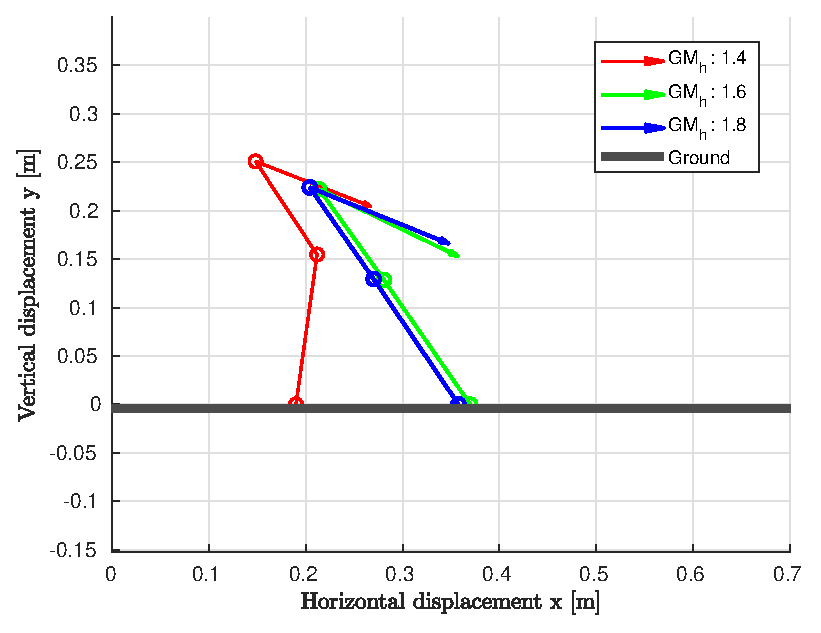
\includegraphics[width=\linewidth]{velocity-vectors/touchdown/velocity-vectors-touchdown.eps}
        \caption{The velocity vectors at touchdown. From this it can be seen that the robot performs the touchdown with a fully extended knee if$~\gls{GM}_h \geq 1.6$, as the three circles representing the joints form a straight line.}%
        \label{fig:velocity-vectors-touchdown}%
        \vspace*{2mm}%
    \end{subfigure}%
    %
    \vfil%
    %
    \centering%
    \begin{subfigure}[b]{0.8\linewidth}%
        \centering%
        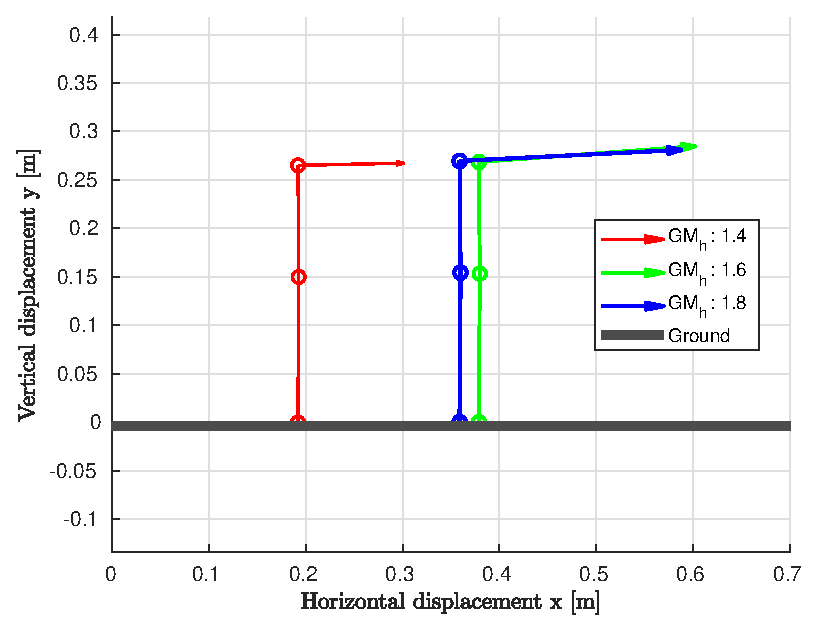
\includegraphics[width=\linewidth]{velocity-vectors/vlo/velocity-vectors-vlo.eps}
        \caption{The velocity vectors at~\glsxtrshort{vlo}$_{1}$,~\ie after a single step is completed, the swing leg attains ground contact and the~\glsxtrshort{com} is orthogonally above the second foot point ($\gls{x}_{\glsxtrshort{com}} = \gls{x}_{FP_2}$).}%
        \label{fig:velocity-vectors-vlo}%
    \end{subfigure}%
    \caption{Velocity vectors at touchdown (\subref{fig:velocity-vectors-touchdown}) and at~\glsxtrshort{vlo}$_{1}$ (\subref{fig:velocity-vectors-vlo}). At the beginning of the velocity vectors the leg position is shown schematically, where the hip, knee and ankle joints are drawn as circles. The colors refer to the different motor gains, with red representing the lowest with a$~\gls{GM}_h$ of 1.4, and blue the highest with a$~\gls{GM}_h$ of 1.8. The velocity vectors are scaled by a factor of 0.15.}%
    \label{fig:velocity-vectors}%
\end{figure}

Figure~\ref{fig:com-horizontal-velocity} shows the trajectory of the horizontal velocity of the~\glsxtrshort{com} during the motion. For legibility purposes, the first $10\,\textrm{\si{\second}}$ of movement are displayed. The robot moves with an average forward velocity of $0.8379\,\textrm{\si{\metre\per\second}}$. The amplitude of the horizontal velocity ranges from a maximum of $1.7803\,\textrm{\si{\metre\per\second}}$ to a minimum of $-0.7106\,\textrm{\si{\metre\per\second}}$. In order to minimize the energy consumption of the system, the amplitude deflection should be reduced and negative forward velocities avoided. The trajectory of the vertical velocity of the~\glsxtrlong{com} during the motion of the robot is shown in appendix~\ref{app:B}.

\begin{figure}[htb]%
    \centering%
    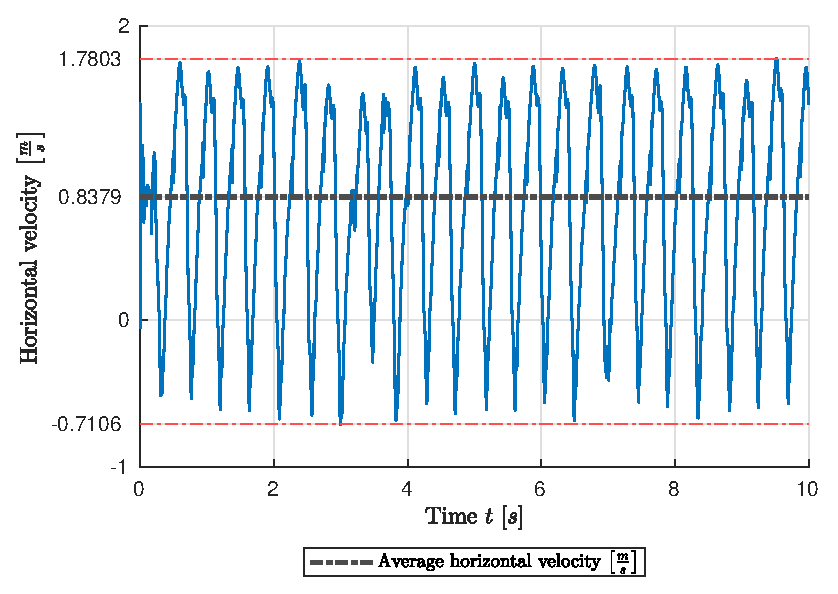
\includegraphics[width=\linewidth]{com-velocity/com-horizontal-velocity.eps}
    \caption{The trajectory of the horizontal velocity of the~\glsxtrlong{com} during the motion. For legibility purposes, the first $10\,\textrm{\si{\second}}$ of movement are displayed. The robot moves with an average forward velocity of $0.8379\,\textrm{\si{\metre\per\second}}$. The amplitude of the horizontal velocity ranges from a maximum of $1.7803\,\textrm{\si{\metre\per\second}}$ to a minimum of $-0.7106\,\textrm{\si{\metre\per\second}}$.}%
    \label{fig:com-horizontal-velocity}%
\end{figure}%
% \noindent

Figure~\ref{fig:phi-hip-torso} shows the angle of the torso ($q_{3}$) and the right hip ($q_{4}$) with respect to the world from~\glsxtrshort{vlo}$_0$ to~\glsxtrshort{vlo}$_1$. The phase of the double support is drawn in blue, the time of the touchdown is in the phase change of the single to the double support and is marked by the dashed line (blue). The torso makes a change of direction at the time of the touchdown,~\ie before the touchdown it falls forwards, while falling backwards again after the touchdown. One cycle of the gait of the JenaFox robot can be seen in figure~\ref{fig:jenafox-vlo}, which starts at the moment of~\glsxtrshort{vlo}$_{0}$ (\subref{fig:jenafox-vlo0}) and ends after one step is completed at~\glsxtrshort{vlo}$_{1}$ of the opposite leg (\subref{fig:jenafox-vlo7}).

\begin{figure}[H]%
    \centering%
    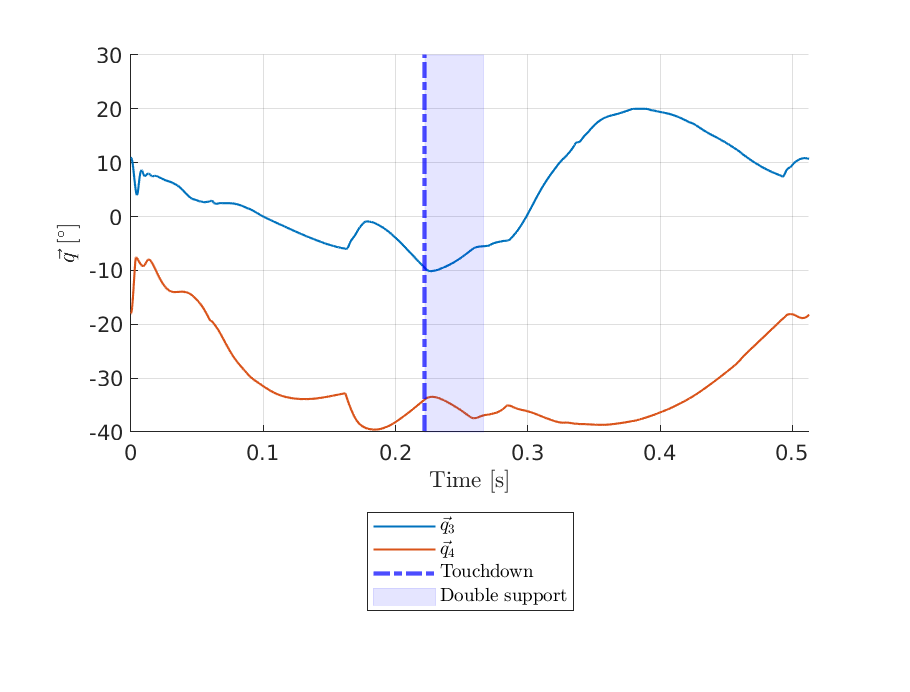
\includegraphics[width=\linewidth]{phi-hip-torso/phi-hip-torso.eps}
    \caption{The angle of the torso ($q_{3}$) and the right hip ($q_{4}$) with respect to the world from~\glsxtrshort{vlo}$_0$ to~\glsxtrshort{vlo}$_1$. The phase of the double support is drawn in blue, the time of the touchdown is in the phase change of the single to the double support and is marked by the dashed line (blue). The torso makes a change of direction at the time of the touchdown,~\ie before the touchdown it falls forwards, while falling backwards again after the touchdown.}%
    \label{fig:phi-hip-torso}%
\end{figure}%
% \noindent

\begin{figure}[H]%
    \centering%
    \begin{subfigure}[t]{0.2\linewidth}%
        \centering%
        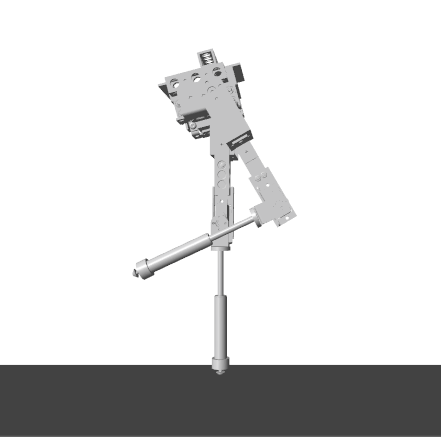
\includegraphics[width=\linewidth]{jenafox/vlo/vlo0.png}
        \caption{\glsxtrshort{vlo}$_{0}$}%
        \label{fig:jenafox-vlo0}%
        % \vspace*{2mm}%
    \end{subfigure}%
    %
    \begin{subfigure}[t]{0.2\linewidth}%
        \centering%
        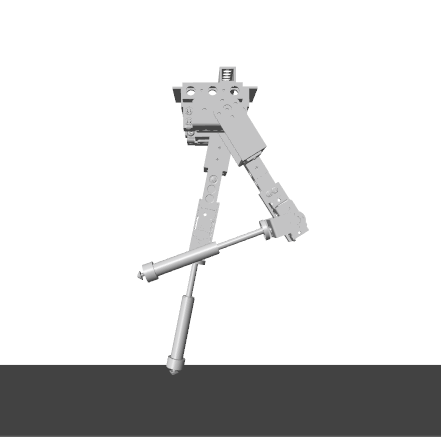
\includegraphics[width=\linewidth]{jenafox/vlo/vlo1.png}
        \caption{Right hip flexion}%
        \label{fig:jenafox-vlo1}%
        \vspace*{2mm}%
    \end{subfigure}%
    %
    \begin{subfigure}[t]{0.2\linewidth}%
        \centering%
        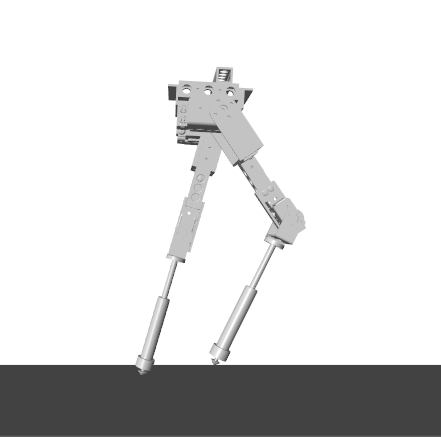
\includegraphics[width=\linewidth]{jenafox/vlo/vlo2.png}
        \caption{Right knee extension}%
        \label{fig:jenafox-vlo2}%
        \vspace*{2mm}%
    \end{subfigure}%
    %
    \begin{subfigure}[t]{0.2\linewidth}%
        \centering%
        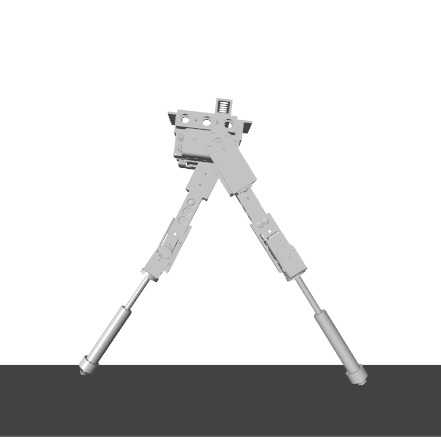
\includegraphics[width=\linewidth]{jenafox/vlo/vlo3.png}
        \caption{Double support}%
        \label{fig:jenafox-vlo3}%
        \vspace*{2mm}%
    \end{subfigure}%
    %
    \vfil
    %
    \begin{subfigure}[b]{0.2\linewidth}%
        \centering%
        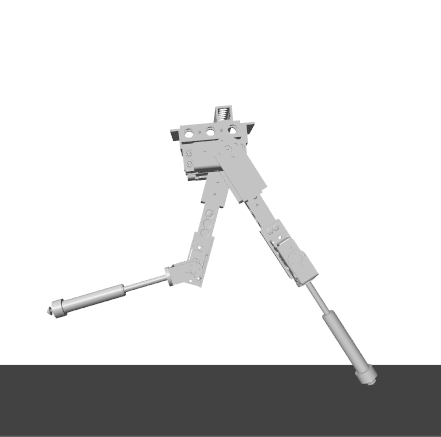
\includegraphics[width=\linewidth]{jenafox/vlo/vlo4.png}
        \caption{Left knee flexion}%
        \label{fig:jenafox-vlo4}%                      
    \end{subfigure}%
    %
    \begin{subfigure}[b]{0.2\linewidth}%
        \centering%
        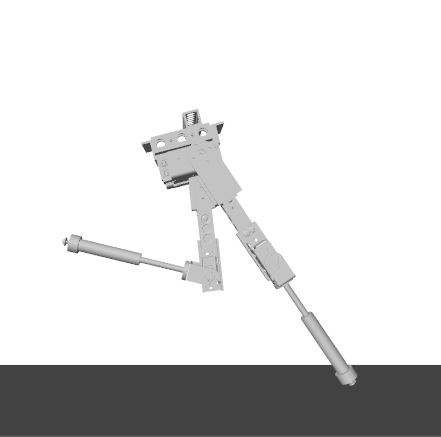
\includegraphics[width=\linewidth]{jenafox/vlo/vlo5.png}
        \caption{Right hip extension}%
        \label{fig:jenafox-vlo5}%                      
    \end{subfigure}%
    %
    \begin{subfigure}[b]{0.2\linewidth}%
        \centering%
        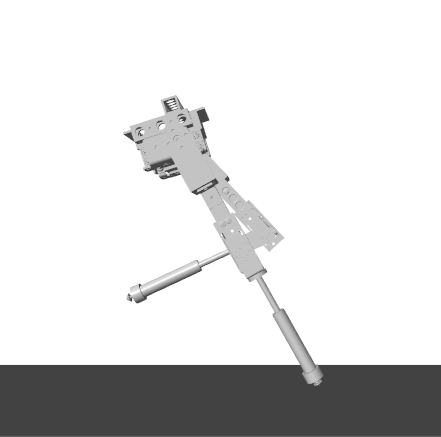
\includegraphics[width=\linewidth]{jenafox/vlo/vlo6.png}
        \caption{Left hip flexion}%
        \label{fig:jenafox-vlo6}%                      
    \end{subfigure}%
    %
    \begin{subfigure}[b]{0.2\linewidth}%
        \centering%
        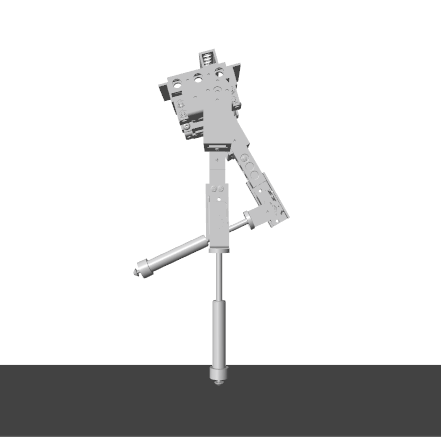
\includegraphics[width=\linewidth]{jenafox/vlo/vlo7.png}
        \caption{\glsxtrshort{vlo}$_{1}$}%
        \label{fig:jenafox-vlo7}%                      
    \end{subfigure}%
    %
    \caption{One cycle of the gait of the JenaFox robot, starting at the moment of~\glsxtrshort{vlo}$_{0}$ (\subref{fig:jenafox-vlo0}) and ending after one step is completed at~\glsxtrshort{vlo}$_{1}$ of the opposite leg (\subref{fig:jenafox-vlo7}).}%
    \label{fig:jenafox-vlo}%
\end{figure}%
% \noindent

% !TeX spellcheck = en_US

\section{Stability Analysis}

A first indicator of the stability of a walking system is the maximum displacement on the ordinate axis, as bigger oscillations tend to be related with poor robustness of the stability of the gait. Figure~\ref{fig:displacement} shows the trajectory of the~\glsxtrshort{com}, with the help of which a first impression of the stability can be gained, as the~\glsxtrshort{com} remains between $\gls{y}_{min}$ and $\gls{y}_{max}$ at every instant. Note that the vertical displacement remains relatively continuous at the upper end, while strong oscillations occur at the lower end. In figure~\ref{fig:displacement-zoom} a section of the vertical displacement is shown, where it can be seen that the robot reaches a negative horizontal displacement at the lower end, causing a loop. This is far from an ideal gait and is extremely energy consuming. \\

A quantitative analysis of the stability of the system can be achieved by evaluating the phase diagram\footnote{A phase diagram typically consists of a set of curves or trajectories that represent the time evolution of the system's state. Each trajectory represents the path that the system would follow in the phase space for a particular set of initial conditions. By plotting multiple trajectories with different initial conditions, it is possible to visualize the range of possible behaviors of the system.~\cite{Goswami1996}}. In a phase plot, each point in the phase space represents a unique state of the system, defined by the values of its state variables. If during each step the trajectory of the system in the phase plot tends to the limit cycle\footnote{The limit cycle is a type of behavior exhibited by some dynamical systems, in which the system oscillates or repeats its behavior indefinitely, but without necessarily converging to a steady state or equilibrium~\cite{Goswami1996}.}, the system is stable,~\ie the system will converge to the limit cycle regardless of the initial conditions, and the limit cycle will persist indefinitely. In an unstable limit cycle, on the other hand, the trajectory will approach the limit cycle for some initial conditions, but it will diverge from it for others. The existence of a limit cycle in the phase plot thus ensures (marginal) stability.~\cite{Goswami1996} Figure~\ref{fig:phase-plot} shows the phase plot of the simulation,~\ie the graphical representation of the behavior of the dynamical system in the phase space\footnote{The phase space refers to the set of all possible states of a system.}. The plot shows the position of the torso of the JenaFox robot on the sagittal plane (\ie the plane spanned between the abscissa axis (X-axis, orange) and ordinate axis (Y-axis, green), see figure~\ref{fig:coordinate-system}) during its motion and reveals that the robot is asymptotically stable in its gait. The simulation was stopped as soon as the robot reached a distance of $15\,\textrm{\si{\metre}}$. The vertical displacement of the torso in$~\left[\si{\metre}\right]$ is plotted on the abscissa axis, the vertical velocity in$~\left[\si{\metre\per\second}\right]$ on the ordinate axis, respectively.

\begin{figure}[H]%
    \centering%
    \begin{subfigure}[t]{0.74\linewidth}%
        \centering%
        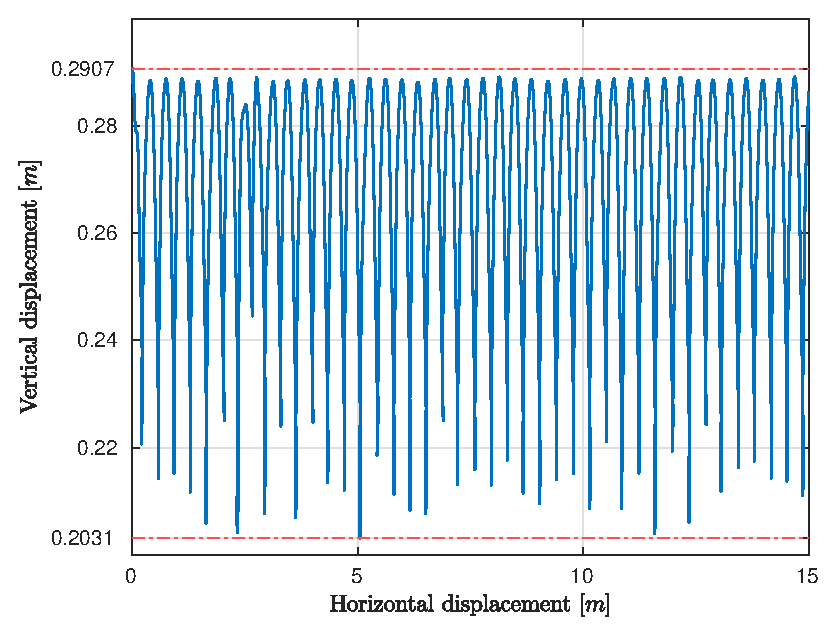
\includegraphics[width=\linewidth]{displacement/displacement.eps}
        \caption{The full trajectory of the~\glsxtrshort{com} over the course of $15\,\textrm{\si{\metre}}$. Note that the vertical displacement remains relatively continuous at the upper end, while strong oscillations occur at the lower end.}%
        \label{fig:displacement-full}%
        \vspace*{2mm}%
    \end{subfigure}%
    %
    \vfil%
    %
    \begin{subfigure}[b]{0.74\linewidth}%
        \centering%
        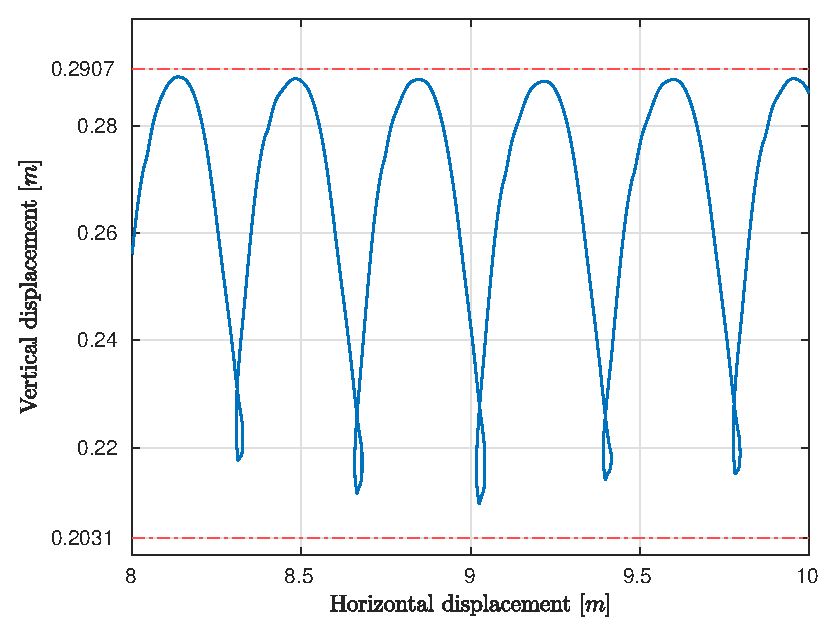
\includegraphics[width=\linewidth]{displacement/displacement-zoom.eps}
        \caption{A section of the~\glsxtrshort{com} trajectory is shown, where it can be seen that the robot reaches a negative horizontal displacement at the lower end, causing a loop. This is far from an ideal gait and is extremely energy consuming.}%
        \label{fig:displacement-zoom}%                      
    \end{subfigure}%
    %
    \caption{The trajectory of the~\glsxtrfull{com}, with the help of which a first impression of the stability can be gained, as bigger oscillations tend to be related with poor robustness of the stability of the gait. The simulation was stopped after a distance of $15\,\textrm{\si{\metre}}$ was reached (\subref{fig:displacement-full}). A more detailed section of the trajectory reveals a negative horizontal displacement at the lower end (\subref{fig:displacement-zoom}). The horizontal displacement of the torso in$~\left[\si{\metre}\right]$ is plotted on the abscissa axis, the vertical displacement in$~\left[\si{\metre}\right]$ on the ordinate axis, respectively.}%
    \label{fig:displacement}%
\end{figure}%
% \noindent

\begin{figure}[H]%
    \centering%
    \begin{subfigure}[t]{0.8\linewidth}%
        \centering%
        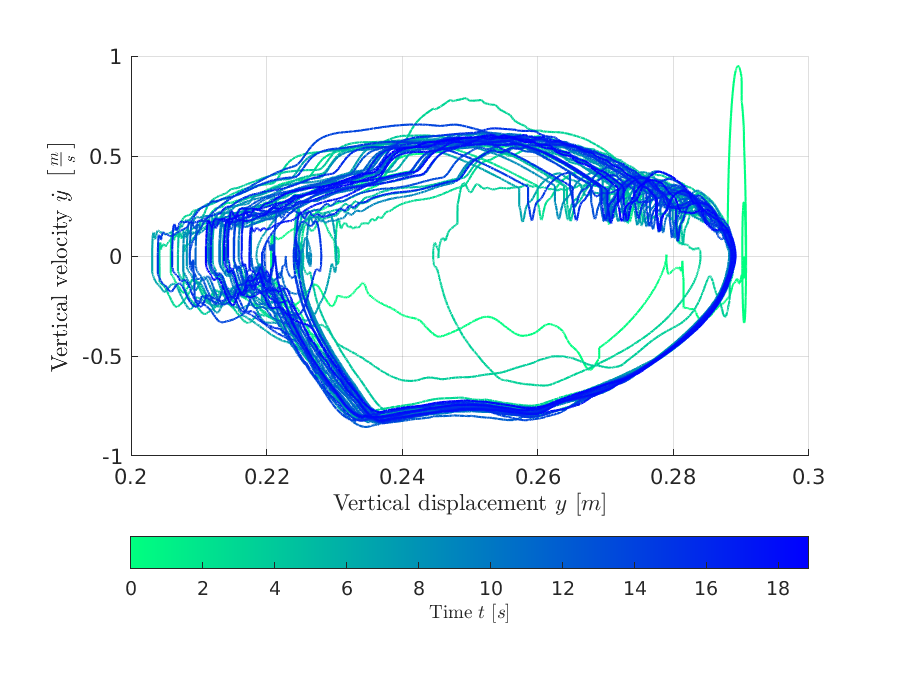
\includegraphics[width=\linewidth]{phase-plot/phase-plot.eps}
        \caption{The phase plot of the simulation. The simulation was stopped after a distance of $15\,\textrm{\si{\metre}}$ was reached. Time is represented by a colormap, which shows that the robot converges to an asymptotically stable gait with few oscillations.}%
        \label{fig:phase-plot-time}%
        \vspace*{2mm}%
    \end{subfigure}%
    %
    \vfil%
    %
    \begin{subfigure}[b]{0.8\linewidth}%
        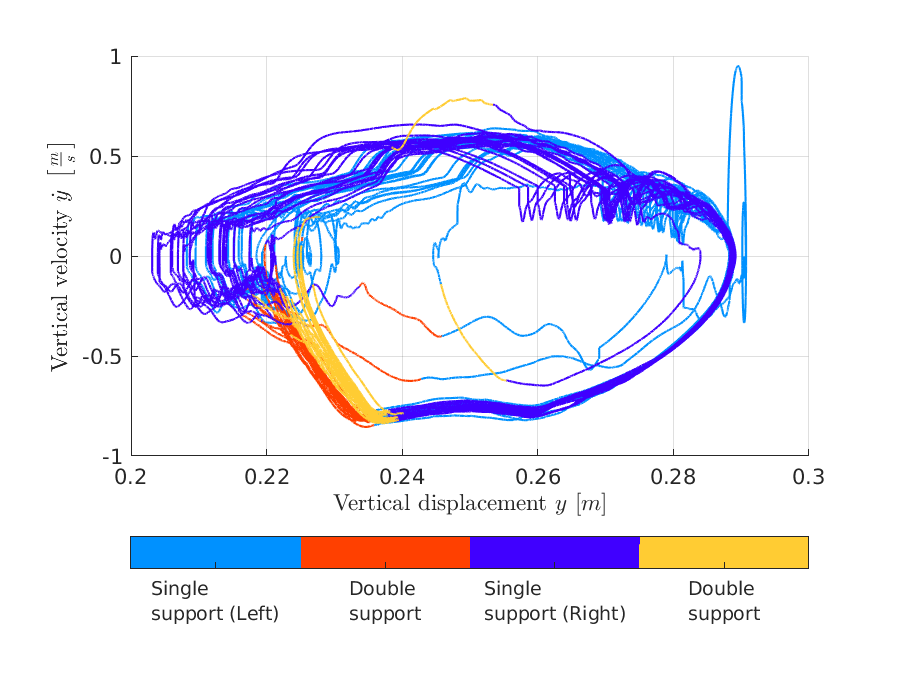
\includegraphics[width=\linewidth]{phase-plot/phase-plot-ground-state.eps}
        \caption{The phase plot of the simulation. The simulation was stopped after a distance of $15\,\textrm{\si{\metre}}$ was reached. The ground state of the system is represented by a colormap, showing the two single support phases (light blue, dark blue) and the two double support phases (red, yellow).}%
        \label{fig:phase-plot-ground-state}%
    \end{subfigure}%
    %
    \caption{The phase plot of the simulation,~\ie the graphical representation of the behavior of the dynamical system in the phase space over the entire simulation with color-encoded time (\subref{fig:phase-plot-time}) and ground state (\subref{fig:phase-plot-ground-state}). The plot shows the position of the torso of the JenaFox robot on the sagittal plane during its motion and reveals that the robot is asymptotically stable in its gait. The vertical displacement of the torso in$~\left[\si{\metre}\right]$ is plotted on the abscissa axis, the vertical velocity in$~\left[\si{\metre\per\second}\right]$ on the ordinate axis, respectively.}%
    \label{fig:phase-plot}%
\end{figure}%
% \noindent
%

\section{Summary}

This chapter presents the results and evaluates the implemented controller with quantitative parameters based on the~\glsxtrlong{mca}. In the course of this work, most of the parameters were chosen according to appropriate experimental data from~\citeauthor*{Geng2006}~\cite{Geng2006} and the remaining ones were determined by sweeping within a reasonable range. The phase plot reveals that the robot is asymptotically stable in its gait. Compared to mammals from the literature, the~\glsxtrshort{mcot} of the robot is relatively high~\cite{Lee2013}. Although a periodic gait has been found, it is not energy efficient. Studying the velocities, it can be seen that the amplitude deflection of the horizontal velocity is quite large and even becomes negative - resulting in a negative horizontal displacement of the robot with a consequently high energy consumption, which should be addressed in further work.